\section{Recherche zum Stand der Kunst}
\label{sec:recherche} Für die Recherche zu den verschiedenen Teilaufgaben ist
die Dokumentation der Open Source Plattform 3D Slicer eine wichtige Ressource
\cite[vgl.]{[}]{slicer2024}. Diese zeigt bereits etablierte Verfahren und einen \textit{Best
Practise} Ansatz. Auch das \citet{extensionsIndex2024} Repository ist eine
wichtige Quelle, da so ein Einblick in andere Lösungen möglich ist. So kommt es,
das nach ausführlicher Recherche zu den Teilaufgaben UI-Design, Pseudo-Extension,
Kapselung Hoffmann, Speicherung Parameter, Dokumentation und Test bereits Lösungen
existieren. Bei diesen Lösungen handelt es sich jedoch nicht um konkrete
Ergebnisse, sondern vielmehr um einen Leitfaden zur Lösung der Teilaufgabe. Die
Recherche hat demnach ergeben, dass diese Teilprobleme im Kontext der 3D Slicer Umgebung,
nicht das erste Mal zutage treten und Lösungswege existieren.

\begin{minipage}{0.40\textwidth}
	Für ein \textbf{UI Design} wird sehr empfohlen, bereits etablierte 3D Slicer Extensions
	als Orientierung zu nutzen. Eine sehr gute Orientierung bietet das Modul
	\textit{Transforms}, das in Abbildung \ref{fig:module_example} zu sehen ist. Zu
	Erkennen ist, dass die UI mittels Collapsible Buttons in verschiedenen Gruppen
	unterteilt wird. Ohne in die verschiedenen Gruppen hineinzublicken, lässt sich
	gut abschätzen, welche Parameter wo zu erwarten sind. Dies ermöglicht dem
	Benutzer ein isoliertes Betrachten der unterschiedlichen Funktionen in diesem
	Modul und so eine gute Benutzerfreundlichkeit.
\end{minipage}
\hfill
\begin{minipage}{0.50\textwidth}
	\centering
	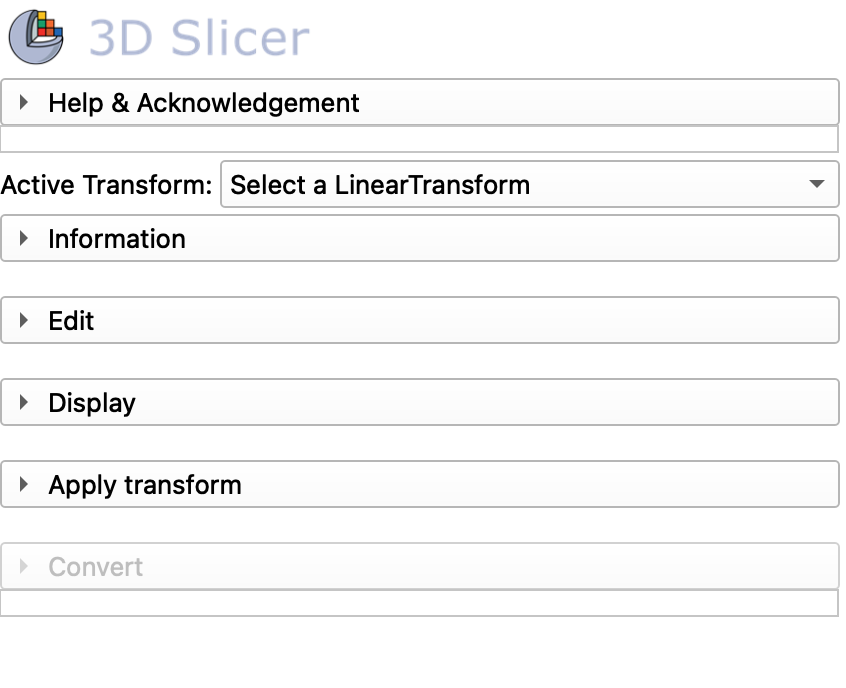
\includegraphics[scale=0.50]{img/modul_example.jpg}
	\captionof{figure}{Das Modul Transforms als Beispiel einer etablierten UI für eine Slicer Extension | Screenshot aus 3D Slicer}
	\label{fig:module_example}
\end{minipage}

Für die Extension, welche in der vorliegenden Arbeit erstellt werden soll, wird genau
dieser Ansatz gepflegt und somit eine gute Benutzbarkeit des Moduls gewährleistet.
Die speziellen wünsche der konkreten Benutzergruppe sollen jedoch nicht zu kurz
kommen.

Für das Erstellen einer \textbf{ersten funktionierenden Extension} bietet Slicer
eine sehr gute Hilfe. 3D Slicer hat hierfür ein eigenes Modul entwickelt, das sich
\textit{Extention Wizard} nennt. Dieses Modul gibt eine gute Einführung in die Entwicklung
mit Slicer. Hiermit lässt sich mittels Leitfaden eine erste Demo Extension
erstellen, die sich bereits gut in 3D Slicer einfügt. Diese Lösung könnte als
Abstraktionsschicht betrachtet werden, da durch dieses Modul im ersten Schritt nahe
zu keine Kenntnisse über die Kernanwendung von Slicer nötig sind. Der
Extentionwizard ist wie folgt zu finden:

\texttt{Modules -> Developer Tools -> Extension Wizard}

Für \textbf{die Kapselung} einer bestimmten Einheit von Code, sieht Slicer eine
Bibliothek innerhalb der Extention vor, so beschreibt es die \citet{slicer2024}.
Das Listing \ref{lst:3d_slicer_projektverzeichnis} zeigt, wo eine Bibliothek
innerhalb einer Extention einzuordnen ist, hier als \texttt{MyLib} zu sehen. Innerhalb
dieses Ordners können sich weitere Module befinden, die als einfache Python-Files
abgelegt werden. Zu beachten ist, dass in jeder Bibliothek eine \texttt{\_\_init\_\_.py}
hinzugefügt wird, sodass dieser Ordner auch entsprechend verwendet werden kann.

\begin{lstlisting}[
    language={python},
    caption={Prinzipeller Aufbau eines Projektes für eine Slicer Extension nach Slicer (2024)},
    label={lst:3d_slicer_projektverzeichnis}]
|-- CMakeLists.txt
|-- MyLib
|   |-- __init__.py
|   |-- cool_maths.py
|   |-- utils.py
|-- MyExtension.py
\end{lstlisting}

Für die Teilaufgabe zur \textbf{Speicherung der Parameter} nutzt Slicer eine
Technik, das durchaus als eines der Kernfunktionen beschrieben werden kann. Die
Rede ist hier von der Klasse \texttt{ParameterNodeWrapper}. Dieser wurde bereits
zu einem früheren Zeitpunkt in dieser Arbeit beschrieben. Für die Funktion dieser
Lösung sei auf den Abschnitt \ref{subsec:benutzerschnitstelle} Benutzerschnittstelle
verwiesen.

Sowohl das \textbf{Benutzerhandbuch}, also auch die technische Dokumentation einer
Slicer Extension wird immer in der \texttt{README.md} des jeweiligen Repository
hinterlegt. In der Extension selber sieht Slicer keine umfangreiche Dokumentation
vor. Es wird lediglich via Link auf die Dokumentation im Repository verwiesen
und eine kurze Einführung gegeben. Auch hier gibt es wieder etablierte Designs,
die als Vorlage verwenden werden können. Die \citet{slicer2024} erwähnt hier
unter anderem das Module
\href{https://github.com/lassoan/SlicerSegmentMesher}{SegmentMesher} als gutes
Beispiel.

Für die letzte Teilaufgabe, das \textbf{Testen}, gibt die Dokumentation von 3D Slicer
ebenfalls eine konkrete Struktur vor. Ist also nicht nötig eigenen Verfahren zu
entwickeln. Für die Softwaretests stell Slicer eine eigene Klasse innerhalb der Slicer
Bibliothek bereit, die alle wichtigen Funktionen enthält, um konkrete Testfälle zu
schreiben. Die Klasse trägt den Namen \textsl{ScriptedLoadableModuleTest} und kann
als Elternklasse für einen Testfall verwendet werden.

\begin{lstlisting}[
    language={python},
    caption={Aufbau einer Testklasse zum ausführen von Unittest nach \citet{slicer2024}},
    label={lst:3d_slicer_test_class}]
class MyExtensionTest(ScriptedLoadableModuleTest)
    def setUp(self):
      # do something befor a test
    def runTest(self):
      # execute your test case here
    def testMyExtension1(self):
      # write your test case here
\end{lstlisting}

Im Listing \ref{lst:3d_slicer_test_class} ist zu sehen, dass sich die Klasse in drei
Teil aufteilt, die Methode \texttt{setUp()}, die als Vorbedingung dient, die Methode
\texttt{runTest()}, die über die UI getriggert werden kann, um die Test zu
starten und die konkreten Textfälle, die in selbst definierten Methoden geschrieben
werden können. Als Beispiel sie hier die Methode \texttt{testMyExtension1()} gezeigt.

Im Laufe dieses Kapitels wurde klar, dass es für einige der Teilaufgaben bereits
Lösungen oder Lösungsansätze gibt, die zu etwas weniger Entwicklungsarbeit führen.
Jedoch trifft dies nicht auf alle Punkte zu, sodass sich der nächste Abschnitt mit
der Erarbeitung von konkreten Lösungsansätzen für die noch nicht behandelten Teilaufgaben
beschäftigt.
% ---------------------------------------------------------------------------------------

\section{Erarbeiten von Lösungsansätzen}
\label{sec:lösungsansätze} hier geht es um Brainstorming

\textbf{Architekturdesign}

\textbf{Single Prozess}

\textbf{Batch Prozess}

% ---------------------------------------------------------------------------------------

\section{Auswahl von Lösungsansätzen}

TODO

- parameter Node erklären ??? wurde eigentlich schon in den theoretischen Grundlagen
angesprochen

- auf das große Klassendiagramm im Anhang verweisens

- die Seintenanzahl anschauen -> Alex